\section{UPPAAL SMC} \label{sec:smc}
\gls{smc} is one of the newer versions of UPPAAL, it works with statistical model checking for more efficient analyses, as it avoids the exhaustive exploration of the state-space.
Statistical exploration have the added benefit of significantly less memory consumption, meaning that the computer's physical memory is rarely the limit when running a query.
This flexibility allows \gls{smc} to be used in other areas which was previous too memory intensive for other UPPAAL tools\cite{cs_smc}.\\
As mentioned in \myref{sec:upp_cora}, \gls{cora} only support linear rates, \gls{smc} facilitates non-linear rates and differential equations, which makes it possible to implement \gls{kibam}, based on our information from \myref{sec:kibam} this will greatly improve our battery estimations.
\gls{smc} looks similar to previous tools in UPPAAL in form of GUI, but it adds new functionality which will be showcased in the rest of this section.
This will include the probability and simulate queries, and how the results of these queries can be interpreted and understood.

We will use the model in \cref{fig:example} as our example for a query that finds the probability for whether or not a specific location is reachable.
\begin{figure}[H]
	\centering
	\begin{tikzpicture}
	%Locations
	\node [init] (l0) {C};
	\node [location] (l1) [right of=l0, xshift=10mm,yshift=10mm, label={
		[align=left]above right:
		\textcolor{name}{L1}
	}] {};
	\node [location] (l2) [right of=l0, xshift=10mm, yshift=-10mm, label={
		[align=left]below right:
		\textcolor{name}{L2}
	}] {};
	\node [location] (l3) [left of=l0, xshift=-10mm, yshift=-10mm, label={
		[align=left]below left:
		\textcolor{name}{L3}
	}] {};
	\node [location] (l4) [left of=l0, xshift=-10mm, yshift=10mm, label={
		[align=left]above left:
		\textcolor{name}{L4}
	}] {};
	%Edges
	\path[->,black, thick] (l0) edge (l1);
	\path[->,black, thick] (l0) edge (l2);
	\path[->,black, thick] (l0) edge (l3);
	\path[->,black, thick] (l0) edge (l4);
	\end{tikzpicture}
	\caption{Model for showcasing probability}
	\label{fig:example}
\end{figure}

\begin{equation}\label{eq:q1}
Pr[<=1](<> Process.L4)
\end{equation}
With this model in place, we are now able to ask if it can reach a specified location by the query shown in query \ref{eq:q1}.
Pr is a keyword to denote that we want to find the probability, square brackets describe the amount of time to pass. 
It is possible to specify which clock to use by adding the variable name of the clock at the beginning, in between the square brackets.\\
Alternative you can swap out time for discrete steps by using the hash(\#) symbol in place of the clock variable.
The expression to be checked is written within the parentheses.
Process refers to the template, and the diamond (<>) describe that a path can reach location \uppLoc{L4}.
Another option is to use square bracket ([]) which mean that a property must be true for all possible states.
Running query \ref{eq:q1} returns the following probability range [0.18744,0.287382] with a certainty of 95\%, when rounded to one decimal the result is 18.7\%-28.7\%.

The simulate query is another feature introduced in \gls{smc}, it is used to run the modelled system a number of time and capture the values of some specified variables at the same time.
To illustrate this a new model is needed, we will use \cref{fig:showcase01} along with its declarations in \cref{lst:showcase1_declarations}.
Three clock are defined in this example, \uppVar{x}, \uppVar{y}, and, \uppVar{t}.
The model have two locations where it is possible to go from one location to the other when the clock \uppVar{t} is between $[5-10]$.
Depending on the location the clocks \uppVar{x} or \uppVar{y} can be incremented with their respectively rates of 1 and 2.
\begin{figure}[H]
	\begin{lstlisting}[language=my_c, caption={Declarations}, label=lst:showcase1_declarations]
	clock x, y, t;
	\end{lstlisting}
\end{figure}
\begin{figure}[H]
	\centering
	\begin{tikzpicture}
	%Locations
	\node [init] (l0) [label={
		[align=left]left:
		\textcolor{invariant}{x '== 1}\\
		\textcolor{invariant}{\&\& y '== 0}\\
		\textcolor{invariant}{\&\& t <= 10}
	}] {};
	\node [location] (l1) [right of=l0, xshift=20mm, label={
		[align=left]right:
		\textcolor{invariant}{x '== 0}\\
		\textcolor{invariant}{\&\& y '== 2}\\
		\textcolor{invariant}{\&\& t <= 10}
	}] {};
	%Edges
	\path[->,black, thick] (l0) edge[bend left=30] node [midway, above][align=left]{
			\textcolor{guard}{t >= 5}\\
			\textcolor{update}{t = 0}
		} (l1);
	\path[->,black, thick] (l1) edge[bend left=30] node [midway, below][align=left]{
			\textcolor{guard}{t >= 5}\\
			\textcolor{update}{t = 0}
		} (l0);
	\end{tikzpicture}
	\caption{Simple model}
	\label{fig:showcase01}
\end{figure}

We will run both of the queries in \ref{eq:q2} which specifies that the model should be simulated once and five times respectively over the duration of 100 time units.
The queries also captures the value of \uppVar{x} and \uppVar{y}.
\begin{equation}\label{eq:q2}
simulate\ 1\ [<=\ 100]\ \{x,y\}\ \text{and}\ 
simulate\ 5\ [<=\ 100]\ \{x,y\}
\end{equation}

\begin{figure}[!h]
	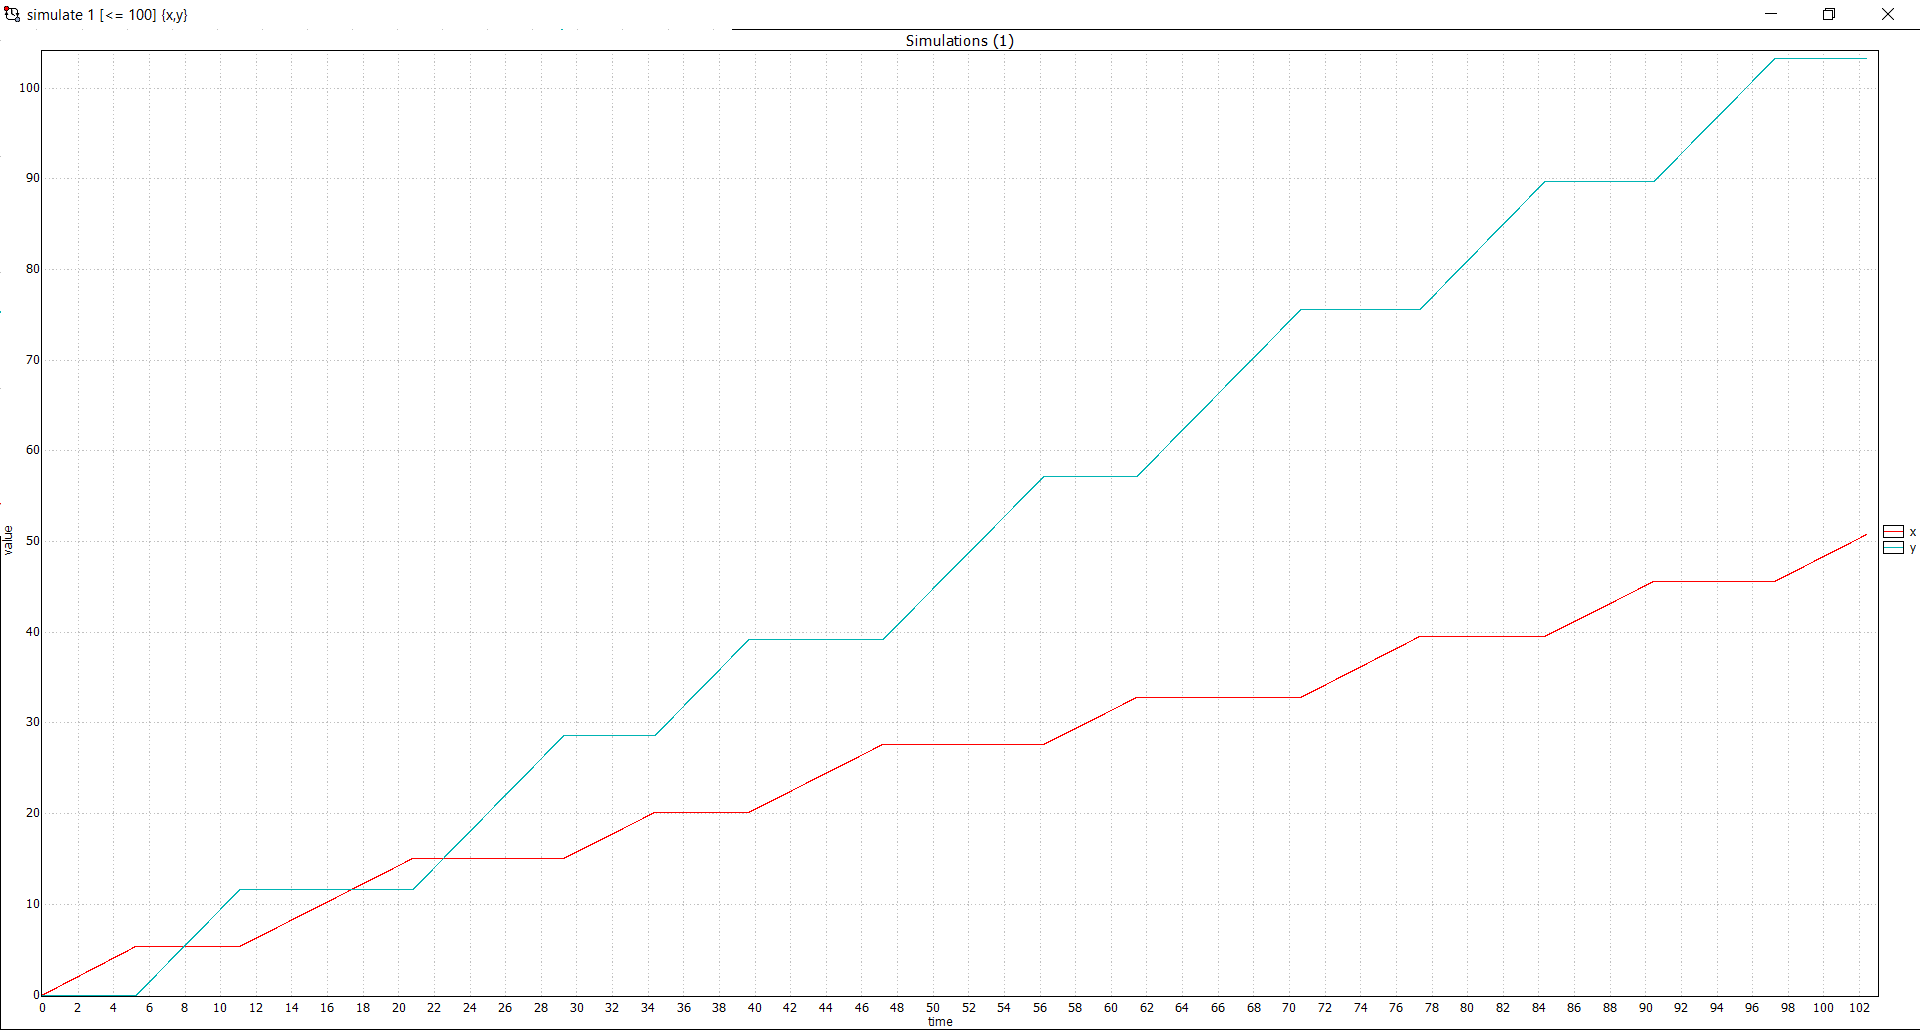
\includegraphics[width=\textwidth]{graphics/showcase01.png}
	\caption{One simulation that captures the value of two variables \uppVar{x, y} over 100 units of time}
	\label{fig:sim01}
\end{figure}

\begin{figure}[!h]
	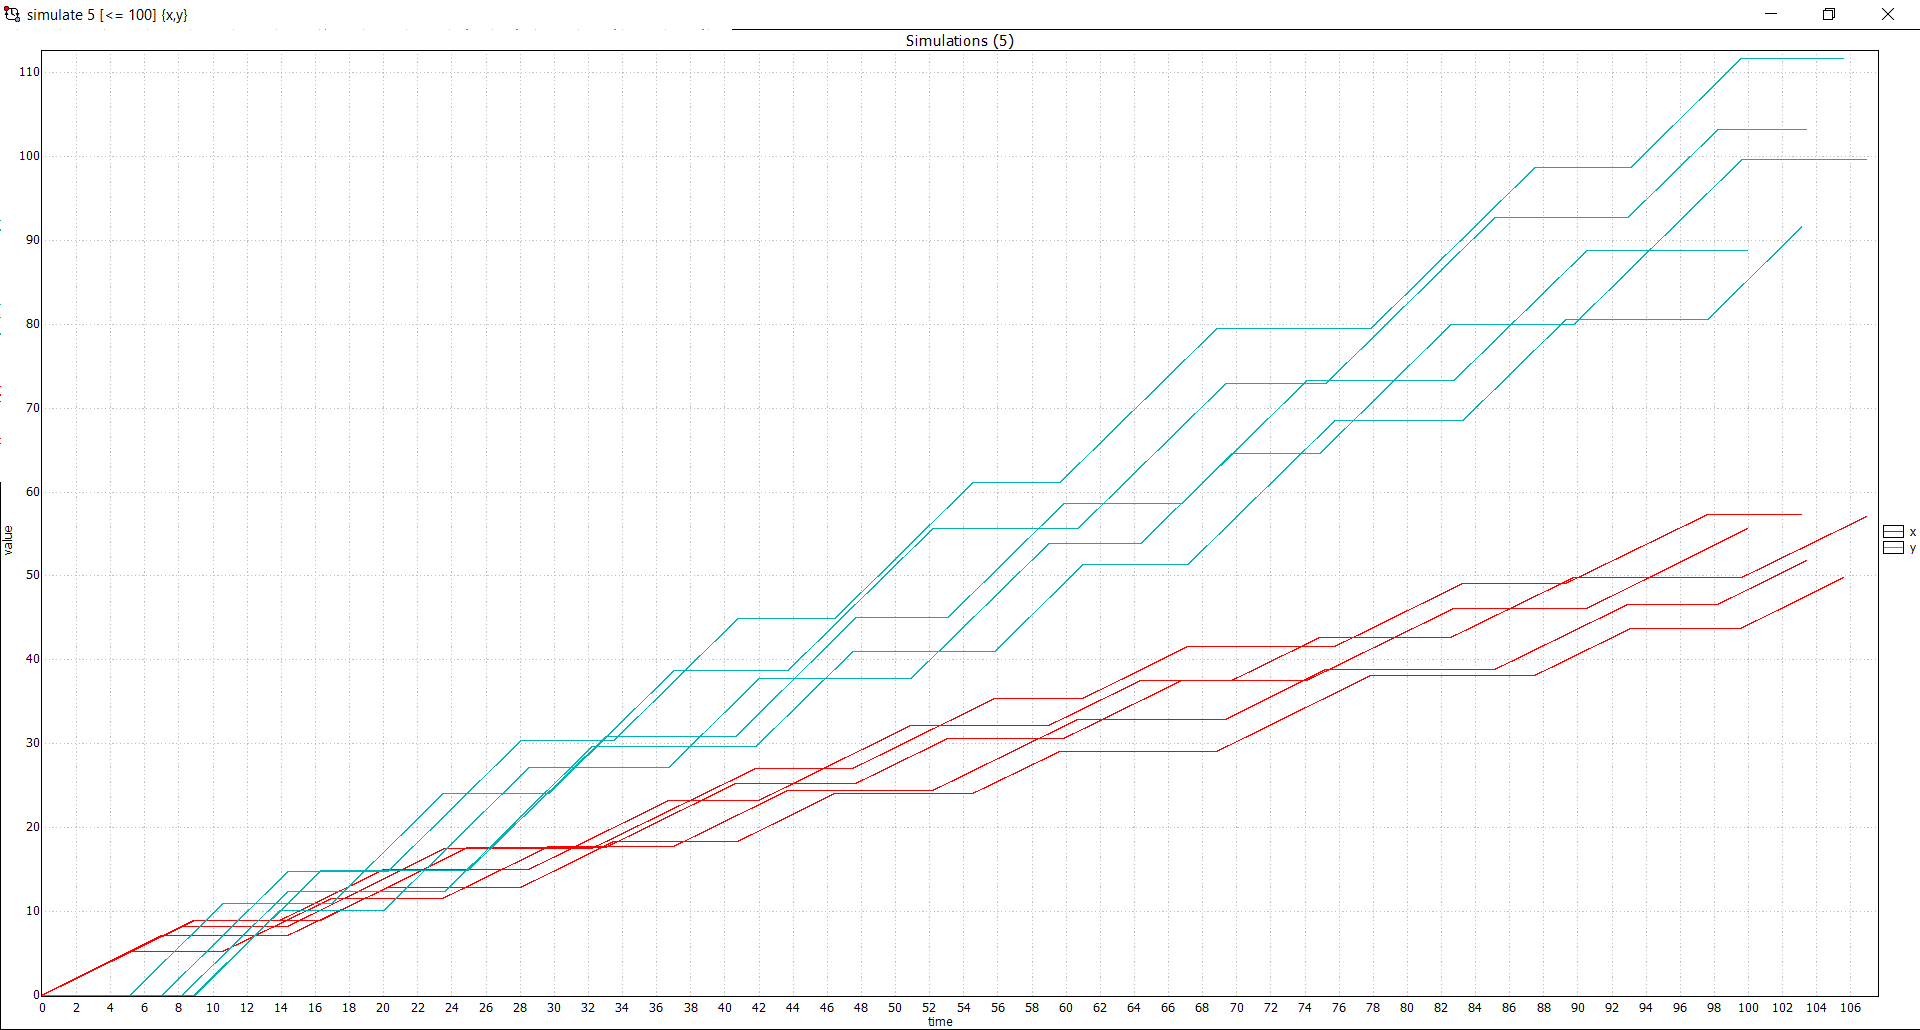
\includegraphics[width=\textwidth]{graphics/showcase02.png}
	\caption{Five simulations that captures the value of two variables \uppVar{x, y} over 100 units of time}
	\label{fig:sim02}
\end{figure}

The result of the two queries is displayed as graphs in \cref{fig:sim01} and \cref{fig:sim02}, where the value axis is the value of \uppVar{x} and \uppVar{y}, and the time axis is the time spent.
Examining the graph we can observe that the value \uppVar{x} tends be about 50 at 100 time units.
From that results a new question can be raised \textit{``What is the probability that \uppVar{x} is above or equal to 50 when 100 time units have passed?''} in \ref{eq:q3} a query have been constructed to answer the question.
\begin{equation}\label{eq:q3}
Pr[<=150](<>\ x\ >=\ 50)
\end{equation}

Like the previous probability example, the query results in a range that describes the probability that \uppVar{x} will be higher or equal to 50 when 150 time units have passed, which in this case results in about a 98\% to 100\% probability.
It is possible to get more information from the query in the form of seven different graphs (Probability Density Distribution, Probability Density Confidence Intervals, Probability Distribution, Probability Confidence Intervals, Cumulative Probability Distribution, Cumulative Probability Confidence Intervals, and Frequency Histogram). 

Frequency Histograms shows the count on the vertical axis and run duration in time on the horizontal axis, each of the columns represent a time where a number of runs have fulfilled the property.
The first column show that out of the 263 runs, three of them had observed the value \uppVar{x} to be higher or equal to 50 at 80.8 time units.
This histogram show that with a 99\% certainty \uppVar{x} will at the earliest be 50 or higher at 80.8 and latest 112 time units.

\begin{figure}[!h]
	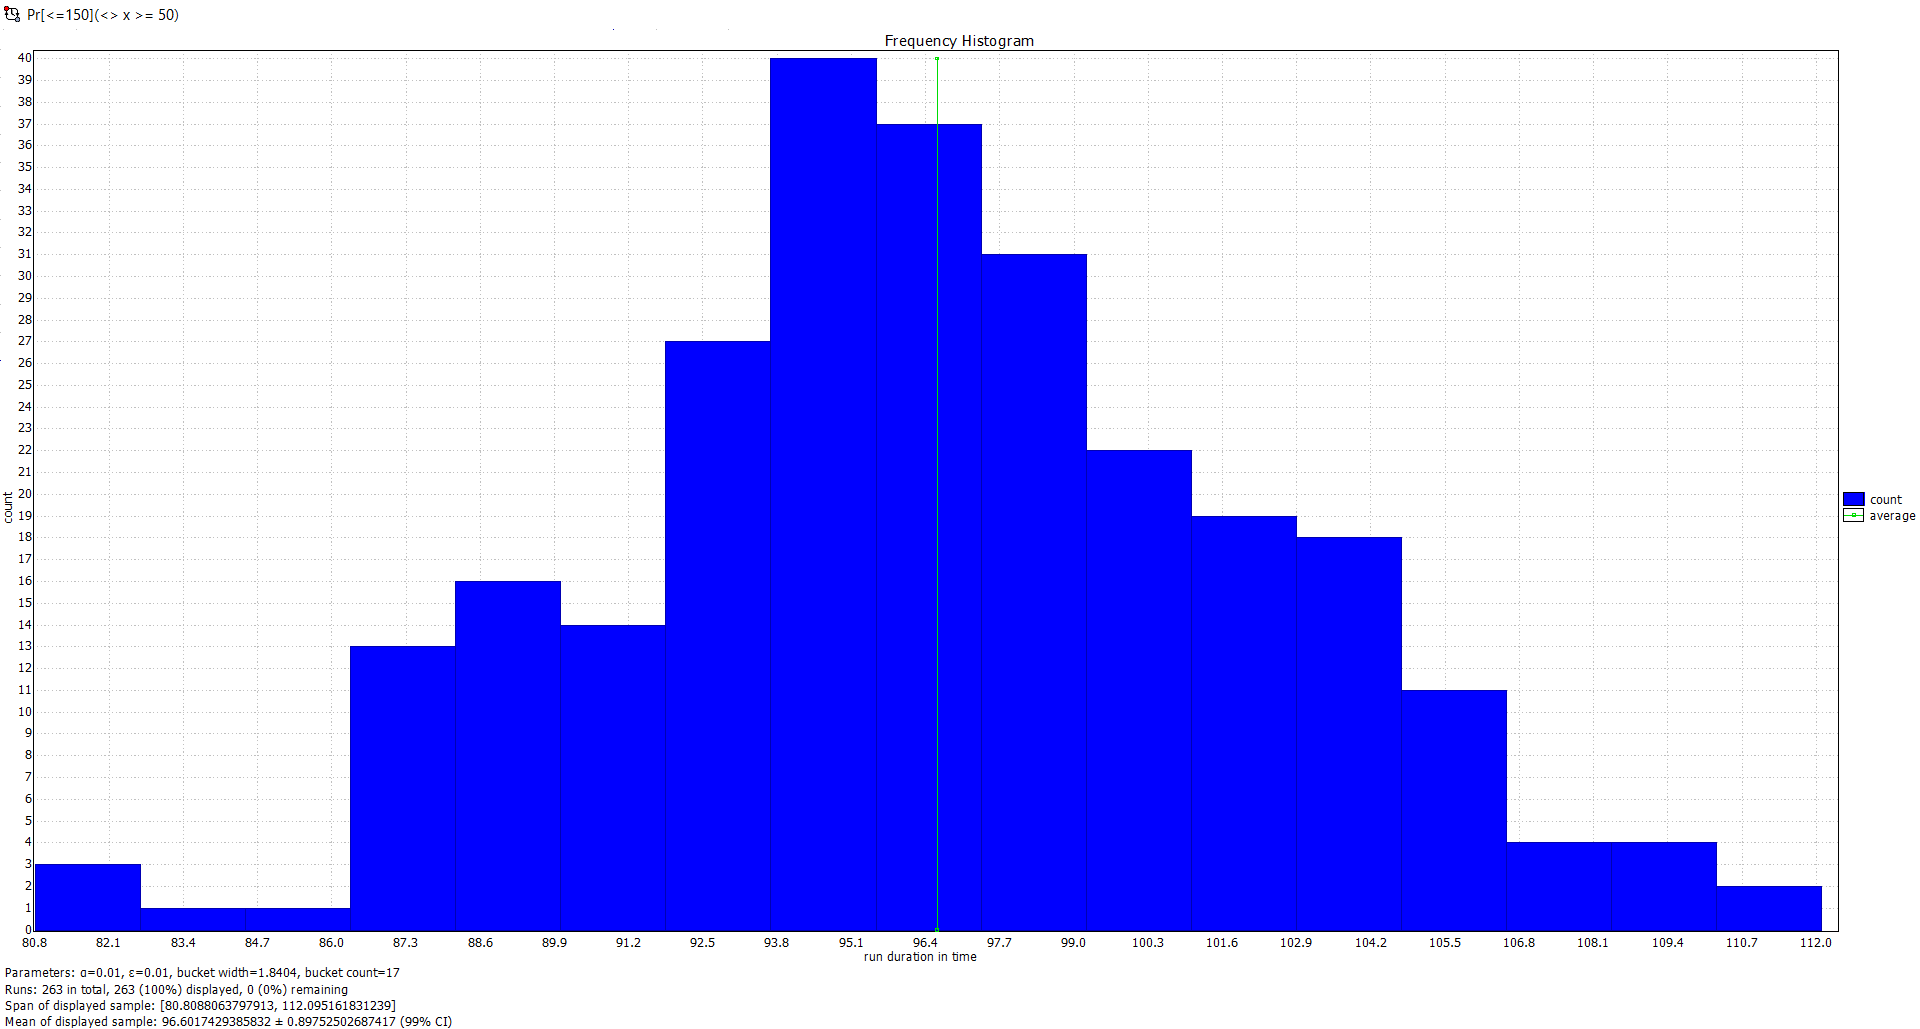
\includegraphics[width=\textwidth]{graphics/eq3fh.png}
	\caption{Frequency histogram generated from query \ref{eq:q3}}
	\label{fig:eq3fh}
\end{figure}

The Cumulative Probability Distribution graph shows the accumulated probability over time.
With a 99\% certainty, at 112 time units there is almost a 100\% probability for \uppVar{x} to be equal or above 50, and at 96.4 time units there is about a 50\% probability.

\begin{figure}[!h]
	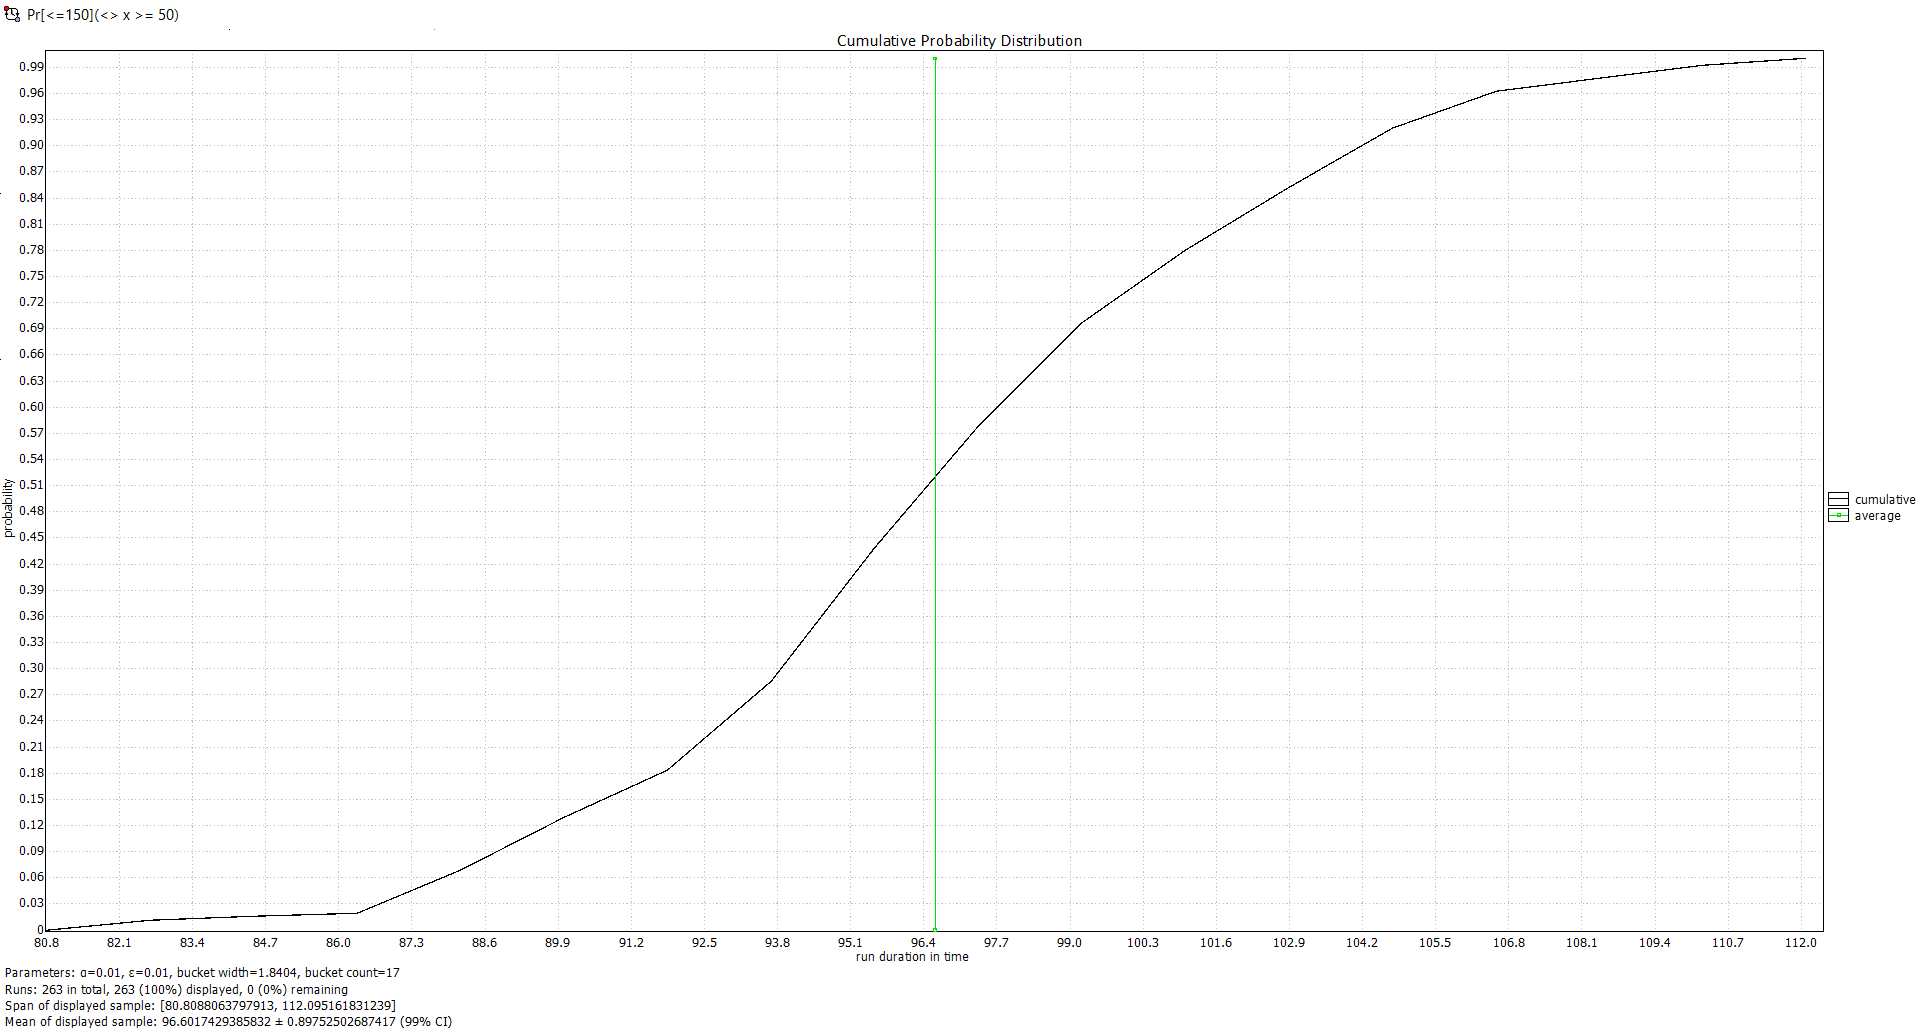
\includegraphics[width=\textwidth]{graphics/eq3cpd.png}
	\caption{Cumulative probability distribution generated from query \ref{eq:q3}}
	\label{fig:eq3cpd}
\end{figure}

The graphs generated by \gls{smc} from the queries can provide useful insight about the probability for a query, an example of this can be seen the above graphs, \cref{fig:eq3fh} \cref{fig:eq3cpd}. 
When running the query it only returns the probability, but the graphs reveal that if we go to 112 or more time units, \uppVar{x} will always be 50 or higher.
